\documentclass[12pt]{beamer}
\usepackage{uglixbeamer}
\title{Notion de complexité}
\subtitle{Algorithmique}
\author{NSI1}

\begin{document}

\maketitle

\begin{frame}{Principe}
\begin{enumerate}[--]
	\item 	on veut résoudre un problème ;\pause
	\item 	celui-ci a une \textit{taille} $n\in\N$ ;\pause
	\item 	on met au point un (ou des) algorithme(s) donnant la solution du problème ;\pause
	\item   on se pose la question suivante :\pause
\end{enumerate}
Mon algorithme est-il \textit{efficace} ?\\\pause

S'il y a plusieurs algorithmes, y en a-t-il un plus efficace que les autres ?
\end{frame}

\begin{frame}{Exemple}
\begin{enumerate}[\textbullet]
	\item 	on dispose d'une liste d'entiers et on veut savoir s'ils sont tous pairs ou non ;\pause
	\item 	notons $n$ la longueur de la liste, c'est la \textit{taille du problème} ;\pause
	\item 	intéressons-nous à 3 algorithmes écrits en \textsc{Python}.
\end{enumerate}
\end{frame}

\begin{frame}[fragile]{Algorithme 1}
	
\begin{minted}{python}
def tous_pairs1(lst: list) -> bool:
    resultat = True
    for x in lst:
        if x % 2 == 1:
            resultat = False
    return resultat
\end{minted}
	
\end{frame}

\begin{frame}[fragile]{Algorithme 2}
    
\begin{minted}{python}
def tous_pairs2(lst: list) -> bool:
    for x in lst:
        if x % 2 == 1:
            return False
    return True
\end{minted}
    
\end{frame}

\begin{frame}[fragile]{Algorithme 3}
    
\begin{minted}{python}
    def tous_pairs1(lst: list) -> bool:
    resultat = True
    for x in lst:
    if x % 2 == 1:
    resultat = False
    return resultat
\end{minted}
    
\end{frame}

\begin{frame}{Questions}
Quel programme semble le plus efficace / inefficace ...\\\pause
\begin{enumerate}[--]
	\item 	en termes d'opérations ?\pause
	\item 	en termes de mémoire ? 	
\end{enumerate}
\end{frame}

\begin{frame}{Réponses}
Il n'y a pas de réponse « absolue » :\pause

\begin{enumerate}[--]
	\item 	Qu'est-ce qu'on considère comme une « opération » ?\pause
	\item 	Comment fonctionne \textit{concrètement} \textsc{Python} ?\\\pause
            (gestion de la mémoire / procédés de calculs)
\end{enumerate}
\end{frame}
\section*{La complexité temporelle}
\begin{frame}{Protocole}
Pour évaluer l'efficacité en terme de nombre d'opérations :\\\pause
\begin{enumerate}[--]
	\item 	On se met d'accord sur ce qu'on considère comme \textit{opération élémentaire} (\textsc{OPEL}).\pause
    \item 	On estime approximativement le temps que prend une \textsc{OPEL} en machine.\pause
	\item 	Seules les \textsc{OPEL} sont considérées comme coûteuses en temps et sont comptabilisées.\pause
    \item   Les autres opérations sont \textit{négligées}.
\end{enumerate}
\end{frame}
\begin{frame}{Complexité moyenne}
On peut « imaginer » une fonction $c_M$ (au sens mathématique du terme) qui \pause
\begin{enumerate}[\textbullet]
	\item 	serait définie pour toute taille $n$ du problème ;\pause
	\item 	donnerait le nombre moyen d'\textsc{OPEL} nécessaires pour résoudre un problème de taille $n$.	\pause
\end{enumerate}
Cette \textit{complexité moyenne} est très rarement calculable (calculs trop compliqués).
\end{frame}

\begin{frame}{Complexité dans le pire des cas}
Plus simple mais tout aussi utile que $c_M$.\\\pause

On cherche pour une taille $n$ donnée le nombre maximal $c(n)$ d'\textsc{OPEL} pour résoudre un problème de cette taille.
\end{frame}

\begin{frame}{Ordre de grandeur}
Quand $n$ augmente, en général, $c(n)$ augmente.\\\pause

Mais à quelle vitesse ?
\end{frame}

\begin{frame}{Vitesses de croissance : graphique} %https://www.geogebra.org/calculator/yhq26vzc
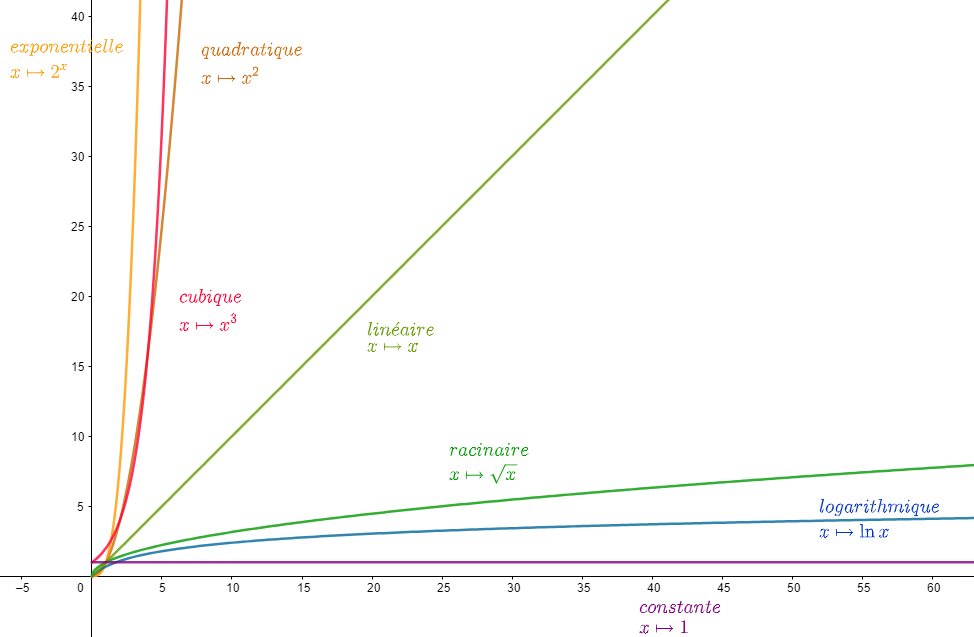
\includegraphics[width=\linewidth]{img/complexite}
\end{frame}

\begin{frame}{Vitesses de croissance : tableau}
Dans la première ligne on a indiqué différentes valeurs de $n$.
\tiny
\renewcommand{\arraystretch}{1.7}
\begin{center}
\begin{tabular}{|c|c|c|c|c|c|c|c|c|}
\hline
\rowcolor{beamerRed}\textbf{\color{white}complexité} & \textbf{\color{white}5} & \textbf{\color{white}10} & \textbf{\color{white}20} & \textbf{\color{white}50} & \textbf{\color{white}250} & \textbf{\color{white}1 000} & \textbf{\color{white}10 000} & \textbf{\color{white}1 000 000} \\
\hline
constante & 10 ns & 10 ns & 10 ns & 10 ns & 10 ns & 10 ns & 10 ns & 10 ns \\
\hline
\rowcolor{blue!10}logarithmique & 10 ns & 10 ns & 10 ns & 20 ns  & 30 ns & 30 ns & 40 ns & 60 ns \\
\hline
racinaire & 22 ns & 32 ns & 45 ns & 71 ns & 158 ns & 316 ns & 1 µs & 10 µs \\
\hline
\rowcolor{blue!10}linéaire & 50 ns & 100 ns & 200 ns & 500 ns & 2,5 µs & 10 µs & 100 µs & 10 ms \\
\hline
quadratique & 250 ns & 1 µs & 4 µs & 25 µs & 625 µs & 10 ms & 1 s & 2,8 h \\
\hline
\rowcolor{blue!10}cubique & 1,25 µs & 10 µs & 80 µs & 1.25 ms & 156 ms & 10 s & 2,7 h & 316 ans \\
\hline
exponentielle & 320 ns & 10 µs & 10 ms & 130 jours & $10^{59}$ ans & ... & ... & ... \\
\hline
\end{tabular}
\end{center}
\end{frame}

\begin{frame}{Bilan}
\Huge 
\begin{center}
La complexité,
c'est important !
\end{center}
\end{frame}

\section*{Retour sur nos algorithmes}

\begin{frame}{Convention}
On décide qu'une \textsc{OPEL} est un accès à un élément d'une liste, ou bien une multiplication.
\end{frame}

\begin{frame}[fragile]{Algorithme 1}
\begin{minted}{python}
def tous_pairs1(lst: list) -> bool:
    resultat = True
    for x in lst:
        if x % 2 == 1:
            resultat = False
    return resultat
\end{minted}

\pause
Quand \texttt{lst} est de taille $n$, il faut $n$ \textsc{OPEL}.\\\pause
L'algorithme est de complexité linéaire.
\end{frame}

\begin{frame}[fragile]{Algorithme 2}
\begin{minted}{python}
def tous_pairs2(lst: list) -> bool:
    for x in lst:
        if x % 2 == 1:
            return False
    return True
\end{minted}

\pause
Dans le meilleur des cas il faut 1 \textsc{OPEL}, $n$ dans le pire des cas.\\\pause
En moyenne il en faut environ 2.
\end{frame}

\begin{frame}[fragile]{Algorithme 3}
\begin{minted}{python}
def tous_pairs3(lst: list) -> bool:
    produit = 1
    for x in lst:
        produit *= x
    if produit % 2 == 1:
        return False
    else:
        return True
\end{minted}
\pause
Puisqu'on parcourt toute la liste, il faut $n$ \textsc{OPEL}...\\\pause
On en rajoute $n$ pour les multiplications...\\\pause 
C'est encore un peu « léger » :  plus $n$ augmentent plus les multiplications prennent du temps...\pause et de la mémoire !
\end{frame}

\begin{frame}[fragile]{Exemple : la fonction \texttt{maximum}}
\begin{minted}{python}
def maximum(lst: list) -> int:
    n = len(lst)
    result = lst[0]
    for i in range(n):
        if lst[i] > result:
            result = lst[i]
    return result
\end{minted}
\end{frame}
\begin{frame}{\textsc{OPEL}}
On convient qu'une \textsc{OPEL} est 
\begin{enumerate}[--]
	\item une affectation ;
    \item une comparaison.
\end{enumerate}
\end{frame}

\begin{frame}[fragile]{Comptabilisation des \textsc{OPEL}}
\begin{minted}{python}
def maximum(lst : list) -> int:
    n = len(lst) # 1 OPEL
    result = lst[0] # 1 OPEL
    for i in range(n): # 1 OPEL
        if lst[i] > result: # 1 OPEL
            result = lst[i] # 1 OPEL
    return result
\end{minted}
\pause
Dans la boucle \pythoninline{for}, qui est itérée $n$ fois, il y a 3 \textsc{OPEL}.\\\pause
Ainsi, la complexité temporelle de la fonction est $3n + 2$.\\
\end{frame}

\begin{frame}{Conclusion}
Quand $n$ est grand, le « $+2$ » n'a guère d'importance et donc cette complexité est presque proportionnelle à $n$.\\\pause 

On dira donc qu'elle est \textit{de l'ordre de n}, ou encore \textit{linéaire}.
\end{frame}

\end{document}